\section{Resultados}

Para evaluar el comportamiento temporal del algoritmo de Gale--Shapley se trabajó con instancias de entrada de tamaños crecientes $N$, desde $32$ hasta $2000$. Para cada valor de $N$ se ejecutó el procedimiento de emparejamiento y se registró el tiempo necesario para realizar únicamente esa fase del proceso, con el fin de centrar el análisis en el costo del algoritmo y no en operaciones auxiliares como la lectura o la impresión.

La Tabla~\ref{tabla:tiempos} muestra los tiempos obtenidos para distintos valores de $N$.

\begin{table}[h]
\centering
\caption{Tiempos de ejecución del algoritmo de Gale--Shapley}
\label{tabla:tiempos}
\begin{tabular}{|c|c|}
\hline
\textbf{N} & \textbf{Tiempo (ms)} \\
\hline
32   & 0.255 \\
64   & 0.694 \\
128  & 2.317 \\
256  & 10.178 \\
384  & 24.806 \\
512  & 41.967 \\
640  & 62.640 \\
768  & 89.410 \\
896  & 119.286 \\
1024 & 215.997 \\
1200 & 220.035 \\
1400 & 332.430 \\
1600 & 405.424 \\
1800 & 532.750 \\
1900 & 586.778 \\
2000 & 646.559 \\
\hline
\end{tabular}
\end{table}

Los datos muestran una tendencia creciente en el tiempo de ejecución conforme aumenta el tamaño de entrada. Por ejemplo, para $N=32$ el tiempo medido fue de $0.255$ ms, mientras que para $N=2000$ se registró un tiempo de $646.559$ ms. Esta diferencia evidencia que el costo del algoritmo aumenta de manera importante al incrementar la dimensión del problema.

Con base en estos resultados se generaron gráficas utilizando escala lineal y escala logarítmica para el eje de $N$, tal como se recomienda en el enunciado de la práctica. La gráfica en escala lineal permite observar con claridad el crecimiento acelerado del tiempo de ejecución, mientras que la representación log-log facilita contrastar el comportamiento observado con un modelo polinómico.
\subsection{Análisis de resultados}

La Figura~\ref{fig:lineal} muestra el tiempo de ejecución del algoritmo en función del tamaño de entrada $N$ en escala lineal. Se observa que el crecimiento no es lineal, sino que aumenta de manera acelerada conforme $N$ se incrementa. Este comportamiento es consistente con una complejidad mayor que $O(N)$.

\begin{figure}[h]
\centering
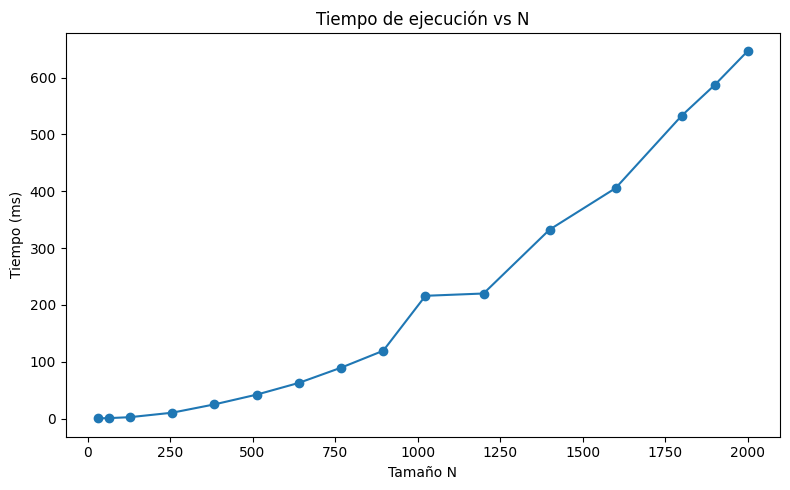
\includegraphics[width=\columnwidth]{figuras/grafica_lineal.png}
\caption{Tiempo de ejecución en escala lineal.}
\label{fig:lineal}
\end{figure}

Para analizar el comportamiento asintótico con mayor claridad, se utilizó una representación log-log, mostrada en la Figura~\ref{fig:loglog}. En esta escala, si el comportamiento sigue una ley polinómica $T(N) = cN^k$, los datos deben aproximarse a una recta cuya pendiente corresponde al exponente $k$.

\begin{figure}[h]
\centering
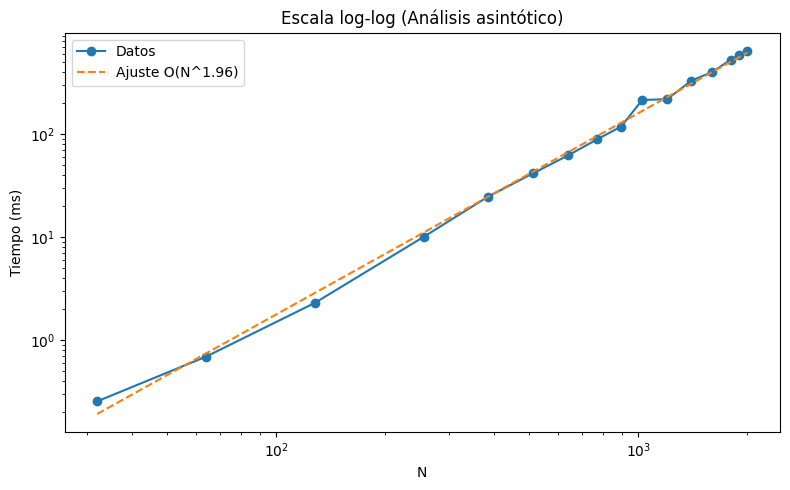
\includegraphics[width=\columnwidth]{figuras/grafica_loglog.png}
\caption{Tiempo de ejecución en escala log-log.}
\label{fig:loglog}
\end{figure}

El ajuste realizado sobre los datos experimentales produjo una pendiente aproximada de $k \approx 1.96$, valor muy cercano al exponente teórico esperado $k = 2$. En consecuencia, los resultados experimentales respaldan que el algoritmo de Gale--Shapley presenta un comportamiento cuadrático $O(N^2)$ en el peor caso. Además, el ajuste obtenido muestra una alta concordancia con la tendencia observada en los datos, por lo que la interpretación no depende de un punto aislado, sino del comportamiento global de la curva.

Las pequeñas desviaciones observadas respecto al ajuste teórico pueden atribuirse a factores propios del entorno de ejecución, como la administración de memoria, la caché del procesador y la sobrecarga del sistema operativo. Por ejemplo, algunos incrementos entre tamaños consecutivos no siguen una proporción exactamente uniforme; sin embargo, estas variaciones locales no modifican la tendencia general de crecimiento.

\subsection{Observaciones}

Los resultados permiten afirmar que la implementación cumple con el comportamiento esperado para este problema. A medida que $N$ crece, el número de propuestas potenciales también aumenta y, por ello, el tiempo de ejecución se incrementa de manera compatible con una función cuadrática.

Asimismo, debe considerarse que las mediciones dependen del entorno experimental y de la instancia utilizada para cada tamaño. Por esta razón, pequeñas fluctuaciones entre valores consecutivos son normales y no contradicen la complejidad teórica del algoritmo. En conjunto, la tabla y las gráficas aportan evidencia suficiente para sostener que la implementación reproduce el desempeño asintótico esperado para Gale--Shapley.
